\cleardoublepage
\begin{refsection}
\chapter{文献综述}

\section{背景介绍}
在计算机视觉领域中,人体姿态估计是指利用计算机视觉的技术来估计图像或视频中人体的空间姿态的任务。这个任务在工业环境与生活环境中均有广泛的应用。在人机交互领域,机器人需要与人类进行合作,机器需要感知人体姿态,以实现更有效的交互;在游戏领域,Microsoft Kinect传感器\cite{shotton2013efficient}使得人类运动姿态捕捉在游戏中的商业应用成为可能;在基于视频的智能监控系统中,对人体的运动姿态的获取能够提供更多的场景中人体的动作及行为信息。

对于三维人体姿态估计,在不同的环境设定下有不同的输入,例如RGB单目输入、RGB双目输入、RGB与深度传感器输入和光学雷达(LiDAR)输入。目前很多人体姿态估计方法对视基于多摄像头或深度传感器的,并已经取得了不错的成果。然而深度传感器如Kinect\cite{kinect}成本较高,需要使用其特殊的设备采集数据。并且Kinect设备设光照影响较大,采集的深度范围有效,难以推广;多摄像头系统需要在固定的场景下,并且需要对多个相机之间的位置进行标定,难以推广到普通场景下;对于目前手机上常用的双目摄像头,其只能在较短距离内提供有效的双目的输入,在大多数距离范围内均只能当作单目摄像头处理。在生活中单目摄像头的产品最为常见,尤其是在网络视频传输、监控摄像头中,单目摄像头的使用便携性是远超过双目摄像头及其他的,并且成本也最低。这也就意味着基于廉价的单目摄像头的人体姿态估计更有应用前景,也就意味着单目RGB图像中进行人体姿态估计的研究更有价值。

许多研究致力于解决图像中人体运动捕获的问题\cite{moeslund2006survey,sminchisescu20073d,brubaker2010video,deva2011_Book,sarafianos20163d}。
这些工作包括单张图片,例如\cite{yang2011articulated,toshev2014deep,chen2014articulated,jain2014learning,tompson2014joint}, 和视频,例如\cite{sapp2011,cherian2014,nie2015joint,park2015articulated,pfister2015flowing,zhang2015human,newell2016stacked} 中的人体姿态恢复。

人体姿态估计问题,一般定义为人体关节点定位问题,即对于输入的图像或视频,通过人体姿态估计的方法得到图像或视频中的人体的关节点的位置,从而得到人体相应的姿态。本课题的研究主要关注的问题为人体的三维姿态估计,即根据输入的视频序列,估计出人体关节的空间坐标。

\section{国内外研究现状}

对视频中的3D单眼姿势估计的早期研究主要集中在用于帧到帧姿势跟踪的生成模型上, e.g.,  \cite{bregler1998tracking,sminchisescu2003kinematic}. 
这些方法依赖于给定的姿势和动态模型来约束姿势搜索空间。
这种方法的显着缺点包括:要求提供初始化,以及无法从跟踪失败中恢复。为了解决这些局限性,在最近的工作中,人们提出了自下而上的模型,例如``松散骨架的人体模型'' \cite{sigal2012loose} 和``通过检测来跟踪'' \cite{andriluka2010monocular}.

另一项研究重点是通过搜索样本数据库\cite{shakhnarovich2003fast,mori2006recovering,jiang20103d,yasin2016dual},或通过学习从图像直接到人类关节位置的映射,来预测3D姿势 \cite{agarwal2006recovering,bo2010twin,salzmann2010implicitly,yu2013unconstrained,ionescu2014human,kostrikov2014depth}。

对于三维人体姿态估计问题,目前的方法主要分为两类:端到端法(end-to-end)\autocite{pavlakos2017coarse}和两步法(two-step)\autocite{zhou2016sparseness}。端到端法(end-to-end)\autocite{pavlakos2017coarse}是指对输入的图像或者视频通过一个卷积网络(ConvNet)的处理直接得到人体的三维姿态;而两步法(two-step)\autocite{zhou2016sparseness}通常是指先根据输入的图像或视频,提取出对应的二维人体姿态,再使用优化的方法或神经网络的方法得到人体的三维姿态。

三维人体姿态估计问题,从相机的数量来分又可以分为单目(single-view)三维人体姿态估计和多目(multi-view)三维人体姿态估计。相比于单目的人体姿态估计,多目的方法可以利用多个视角的额外信息,从而从中提取出更为准确的三维人体姿态,消除单个所带来的深度的不确定性。

从估计的人数上来分,三维人体姿态估计又可以分为单人(single-person)三维人体姿态估计和多人(multi-person)三维人体姿态估计,多人的姿态估计问题相比单人的更加复杂,多人之间的人体互相遮挡与交叉的情况更多,因此也是当前研究的热点所在。


最近,深度卷积网络(CNN)已经成为许多现有技术方法背后的共同元素,包括例如3D人体姿态估计\cite{li20143d,li2015,tekin2015,du2016marker,park20163d,zhou2016deep}。为了应对训练数据的稀缺性,最近的一些工作通过图形渲染\cite{chen2016synthesizing}或图像拼接\cite{rogez2016mocap}来合成训练图像。 

与我们的工作较为密切相关的是:用单个相机捕获的图像序列恢复3D非刚性形状的方法,即运动恢复非刚性结构(NRSFM),\cite{bregler2000recovering,akhter2011trajectory,dai2012simple,zhu2014complex,cho2015complex}, i.e., 运动恢复非刚性结构 (NRSFM),和基于已知骨架\cite{lee1985determination,taylor2000reconstruction,valmadre2010deterministic,park20113d,radwan2013monocular,leonardos2016articulated}或稀疏表示的人体姿势恢复模型。 \cite{ramakrishna2012reconstructing,fan2014pose,akhter2015pose,zhou20153d,zhou2015sparse}. 这些工作的大部分是通过手动标记2D关节位置来实现的。最近的一些工作已经使用2D姿势检测器来自动提供输入关节\cite{simo2012single,wang2014robust},或联合解决2D和3D姿态估计\cite{simo2013joint,zhou2014spatio}。

\subsection{研究方向及进展}
\subsubsection{二维人体姿态估计}
二维人体姿态估计问题,就是从输入图像或视频中,得到在图片上人体的关节点的位置。传统的人体姿态估计的方法对人体结构进行建模,将人体部位的空间相关性用一个树型结构图表示(tree-structured graphical model)\autocite{eichner20122d}。近些年来,深度卷积网络(ConvNet)在二维人体姿态估计问题中取得了重大的进展。早期使用卷积网络(ConvNet)的方法,直接预测人体关节点的坐标\autocite{toshev2014deep},如\refFig{fig:deeppose}所示,这种方式想法直接,但是实际效果并不好。后来人们采用回归热图(heatmaps)\autocite{pfister2015flowing}的方案,来间接预测人体关节点,如\refFig{fig:heatmap}所示。这种方法更适合于卷积网络,它首先在图像上为每个关节点回归一个热图,然后再从中提取出关节点的位置。与直接预测相比,预测热图有以下优点:首先,它避免使用卷积网络来直接预测实际值的问题;其次,它可以处理图像中有多个实例的问题。
\begin{figure}[ht]
    % 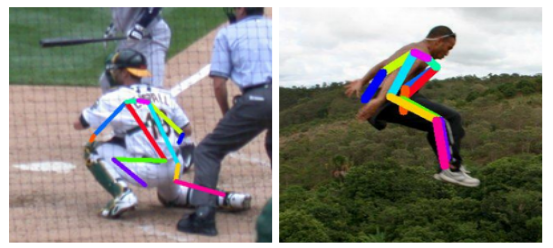
\includegraphics[width=0.32\linewidth]{review/deeppose.png} \hfill
    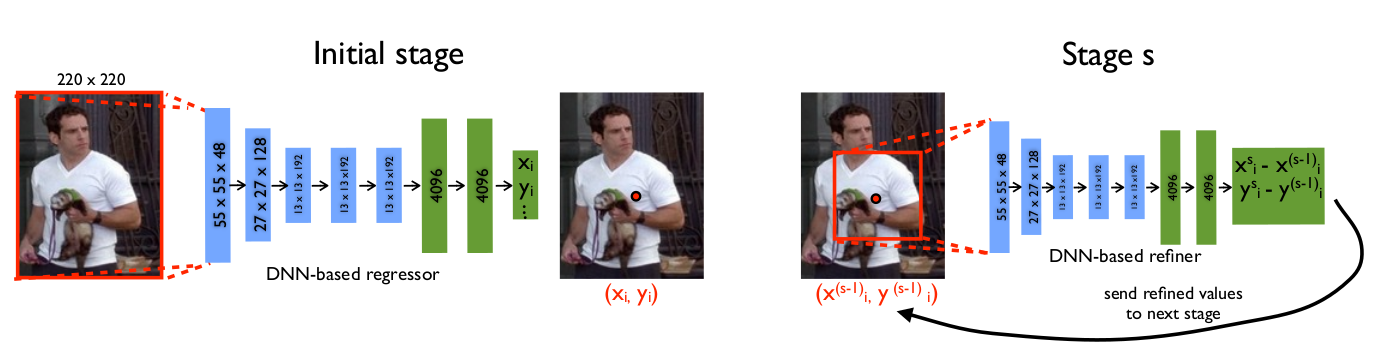
\includegraphics[width=1\linewidth]{review/deeppose_line.png}
    \caption{Deeppose方法\autocite{toshev2014deep}:基于深度神经网络对人体姿态进行回归。左:网络结构可视化,其中蓝色表示卷积层,绿色表示全连接层;右:使用上一阶段的结果取出原图的的部分,对结果进行优化。}\label{fig:deeppose}
\end{figure}
  
\begin{figure}[ht]
    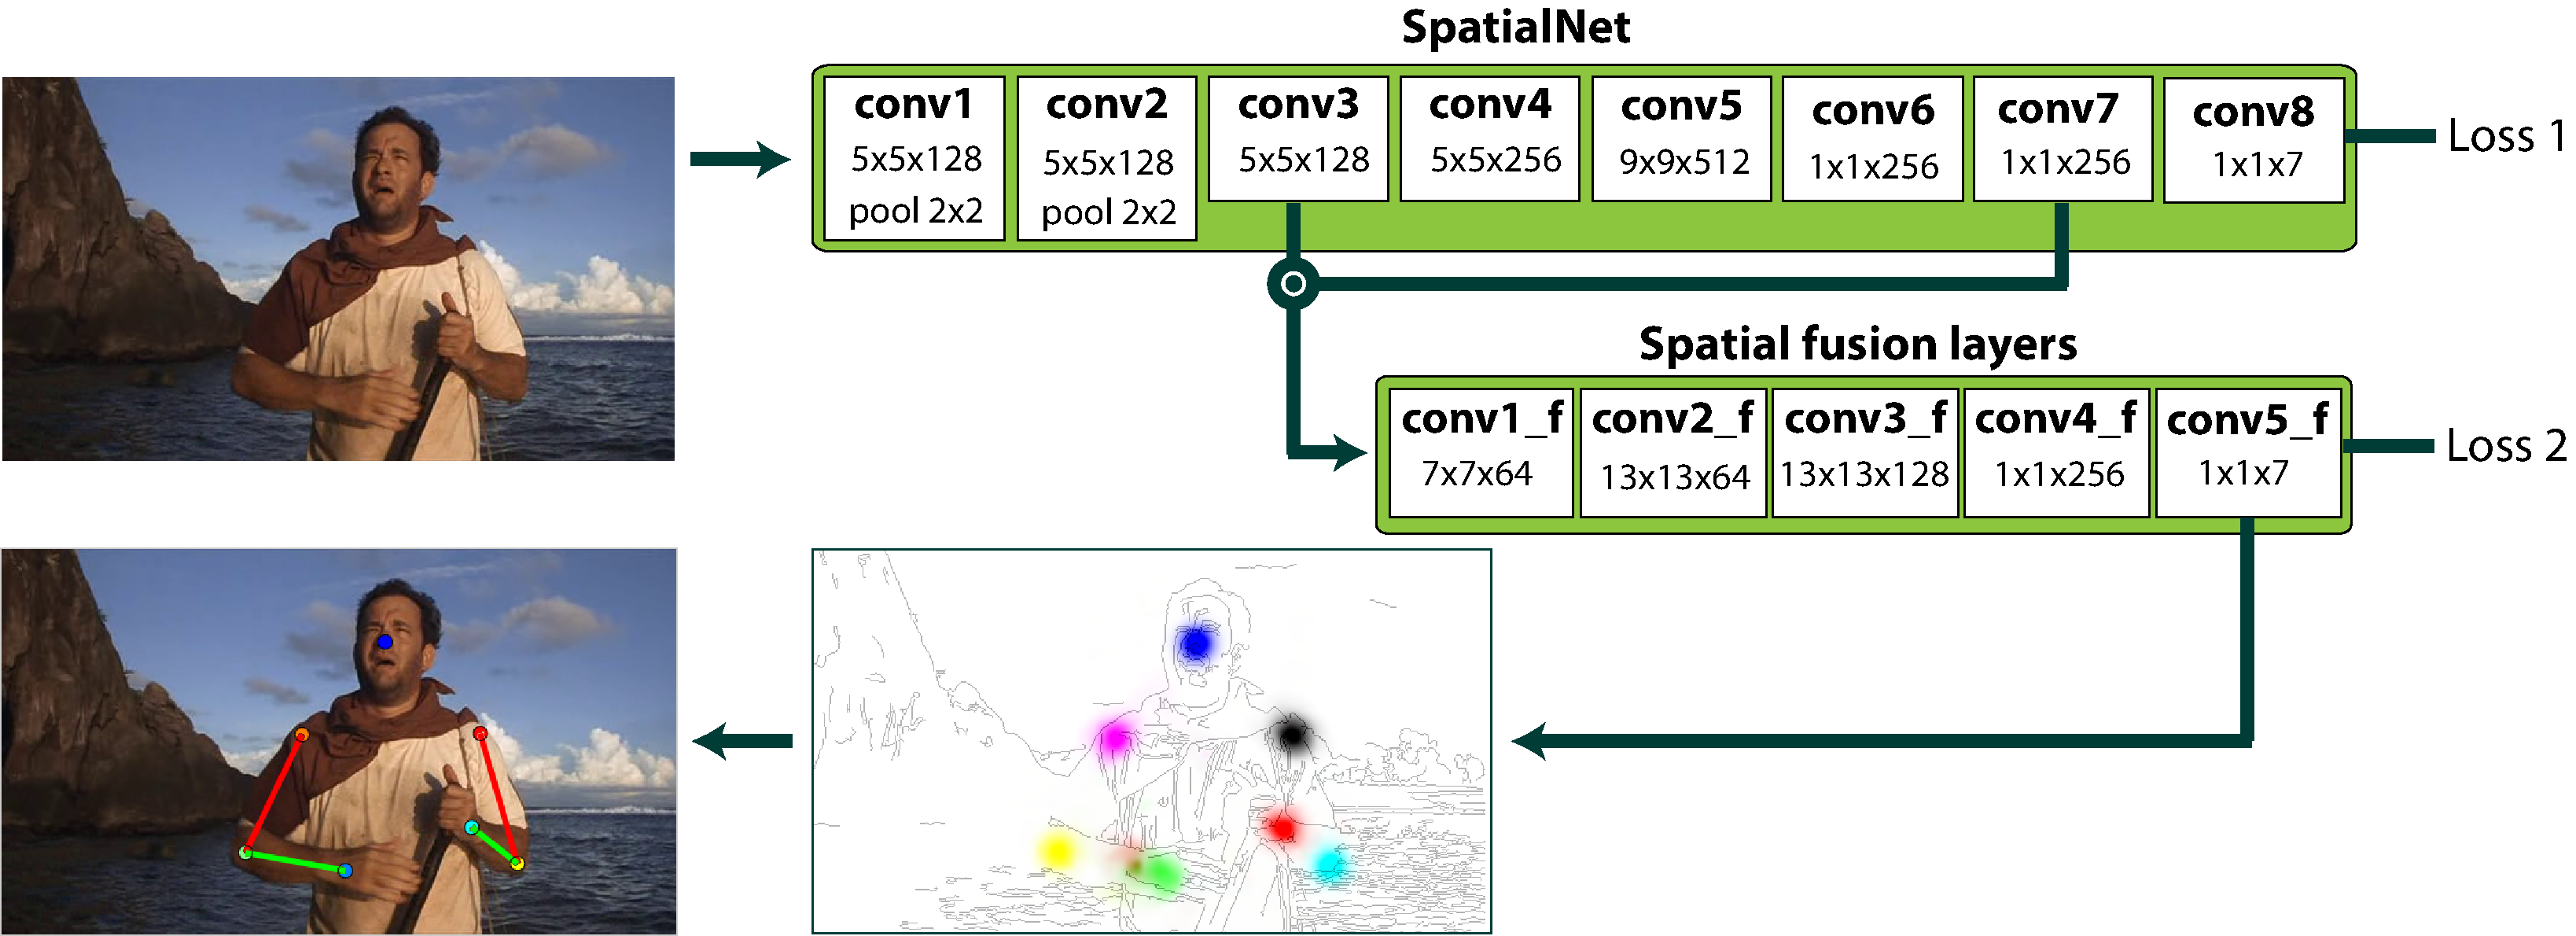
\includegraphics[width=1\linewidth]{review/heatmap.pdf}
    \caption{回归热图\autocite{pfister2015flowing}:对于每一个关节,网络的学习目标是一个热图(heatmap),每个关节的热图是根据关节的真实位置生成的一个高斯分布。同时还通过在不同层次上的特征的混合,使网络学到一个隐式的空间模型。}\label{fig:heatmap}
\end{figure}

在此之后,研究者们设计了许多不同的网络结构,在这一问题上取得了非常好的效果,例如卷积姿势机(Convolutional Pose Machines),堆叠沙漏网络(Stacked Hourglass Networks)\cite{newell2016stacked}。2016年,Stacked Hourglass网络\cite{newell2016stacked}被提出,如\refFig{fig:hourglass}所示。这种网络与之前的结构完全不同,它采用重复的自底向上和自顶向下的漏斗形,并且在中间加入了监督。这样能够利用多个尺度的信息来猜测被遮挡关节的位置,能比级联的效果更好。而之后的很多三维姿态的研究,都是基于这个网络做的。

\begin{figure}[ht]
    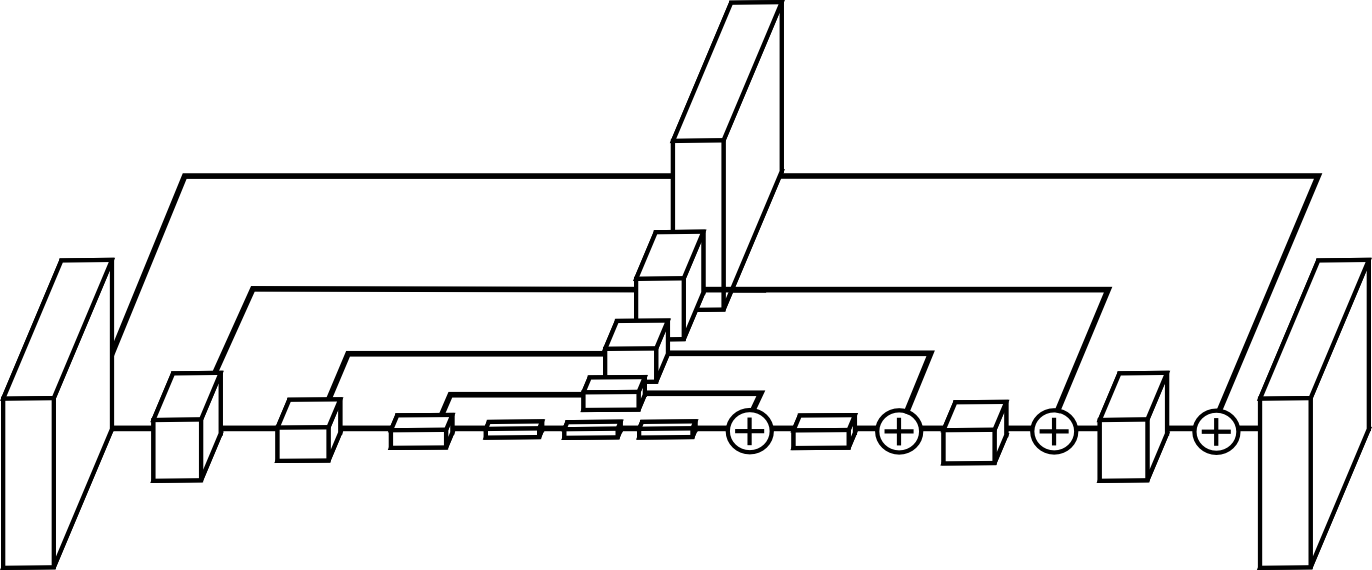
\includegraphics[width=0.4\linewidth]{review/single-hourglass.png}
    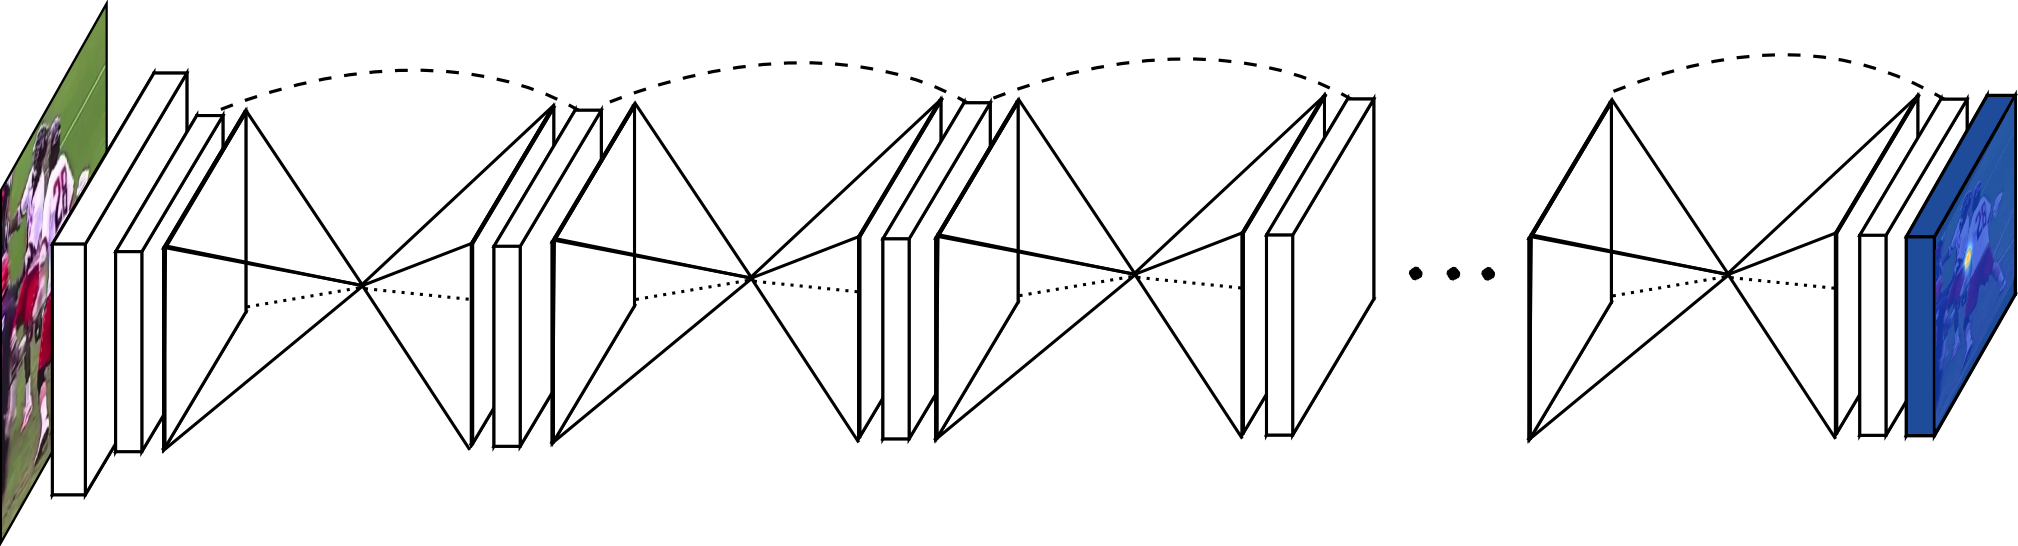
\includegraphics[width=0.59\linewidth]{review/stacked-hg.png}
    \caption{堆叠沙漏网络\autocite{newell2016stacked}:左:单个沙漏网络。使用了连续的下采样与上采样,并将不同步骤的信息混合起来。右:多个沙漏网络串联在一起,能够不断利用前一步的网络输出进行优化}\label{fig:hourglass}
\end{figure}

% \subsection{以深度摄像头作为输入}
% 随着Kinect\autocite{kinect}的推广,深度成像技术取得了明显的进步,并且其成本也越来越低。使用深度相机与传统的相机相比具有许多优势:可以在低光照水平下工作;能够直接给出较为准确的深度估计;具有颜色和纹理不变性。

\subsection{三维人体姿态估计}
目前大部分论文将三维人体姿态估计问题作为从图像或视频中得到人体的主要的关节点的空间位置问题。在这种定义下,三维人体的姿态估计方法可以分为两类:两步法和端到端法。

两步法的主要流程如下:第一步获取人体的二维关节点位置;第二步,从三维动作捕捉的数据集上学习得到人体骨架的先验知识,例如学习一个姿态字典\autocite{zhou2015sparse},如\refFig{fig:twostep}所示。由于从二维到三维的估计具有不确定性,这些方法通过先验知识,例如对四肢长度或骨架的尺寸比例进行假设。两步法的优点是对域的转移更为鲁棒,而且只需要二维动作与三维动作配对的数据集,不需要有图像配对的三维姿态数据集。该方法的缺点是较为依赖二维关节点的检测,在估计二维关节点时如果出错的话恢复出的三维关节点效果就会较差。

\begin{figure}[ht]
    \centering
    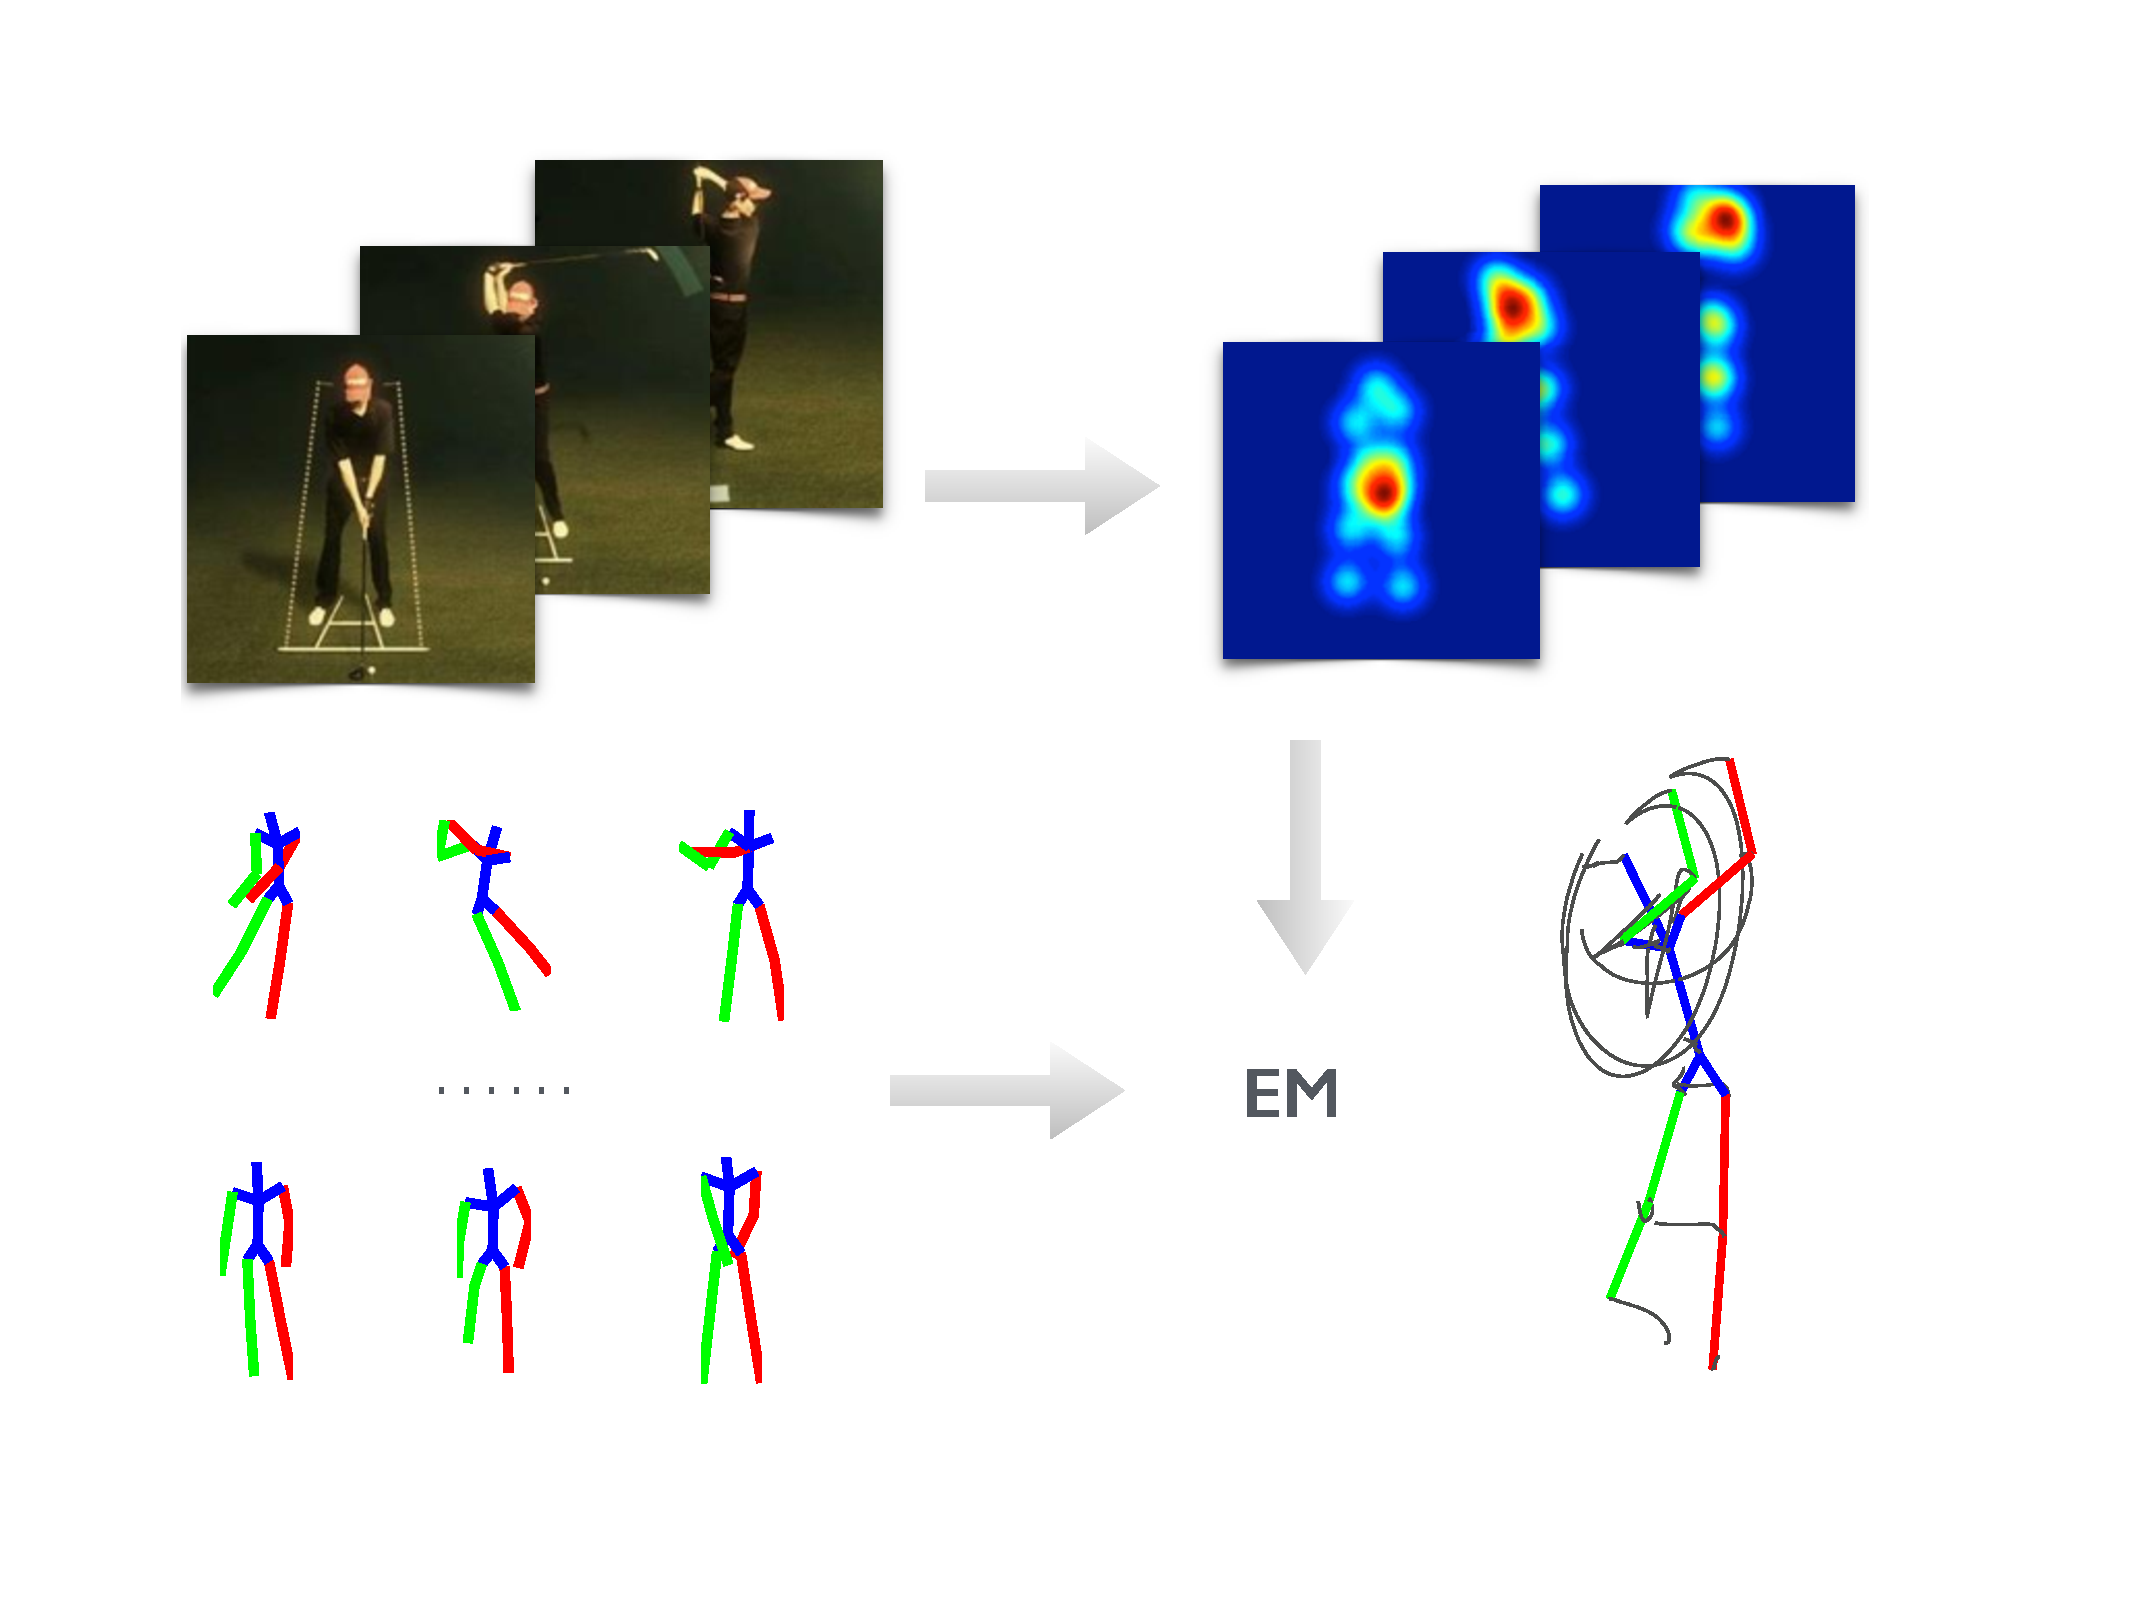
\includegraphics[width=0.4\linewidth]{figures/overview.pdf}
    \caption{两步法\autocite{zhou2015sparse}:先从图片中得到人体的二维姿态,再从二维姿态中恢复三维姿态}\label{fig:twostep}
\end{figure}

从 Toshev \cite{toshev2014deep}等人开始,最近的许多文献的方法,在深度学习框架下直接从输入图像估计得到三维关节点\cite{pavlakos2017coarse}\cite{tekin2017learning}\cite{tome2017lifting}\cite{zhou2017weaklysupervised}。Rogez\cite{rogez2016mocap}等人将人体检测与 3D 人体姿态估计相结合。这种端到端法(end-to-end)的优点如下:能够充分利用输入图像的信息,训练过程简单不需要像两步法(two-step)那样先进行 2D 人体姿态估计,再进行后续处理。但是该方法的缺点也是比较明显的,之前所述的这些直接估计的方法的所使用的具有准确的3D注释的图像均是在受控的动作捕捉系统中捕获。仅在这些受控环境数据集上训练的模型不能很好地泛化到现实世界。

\begin{figure}[ht]
    \centering
    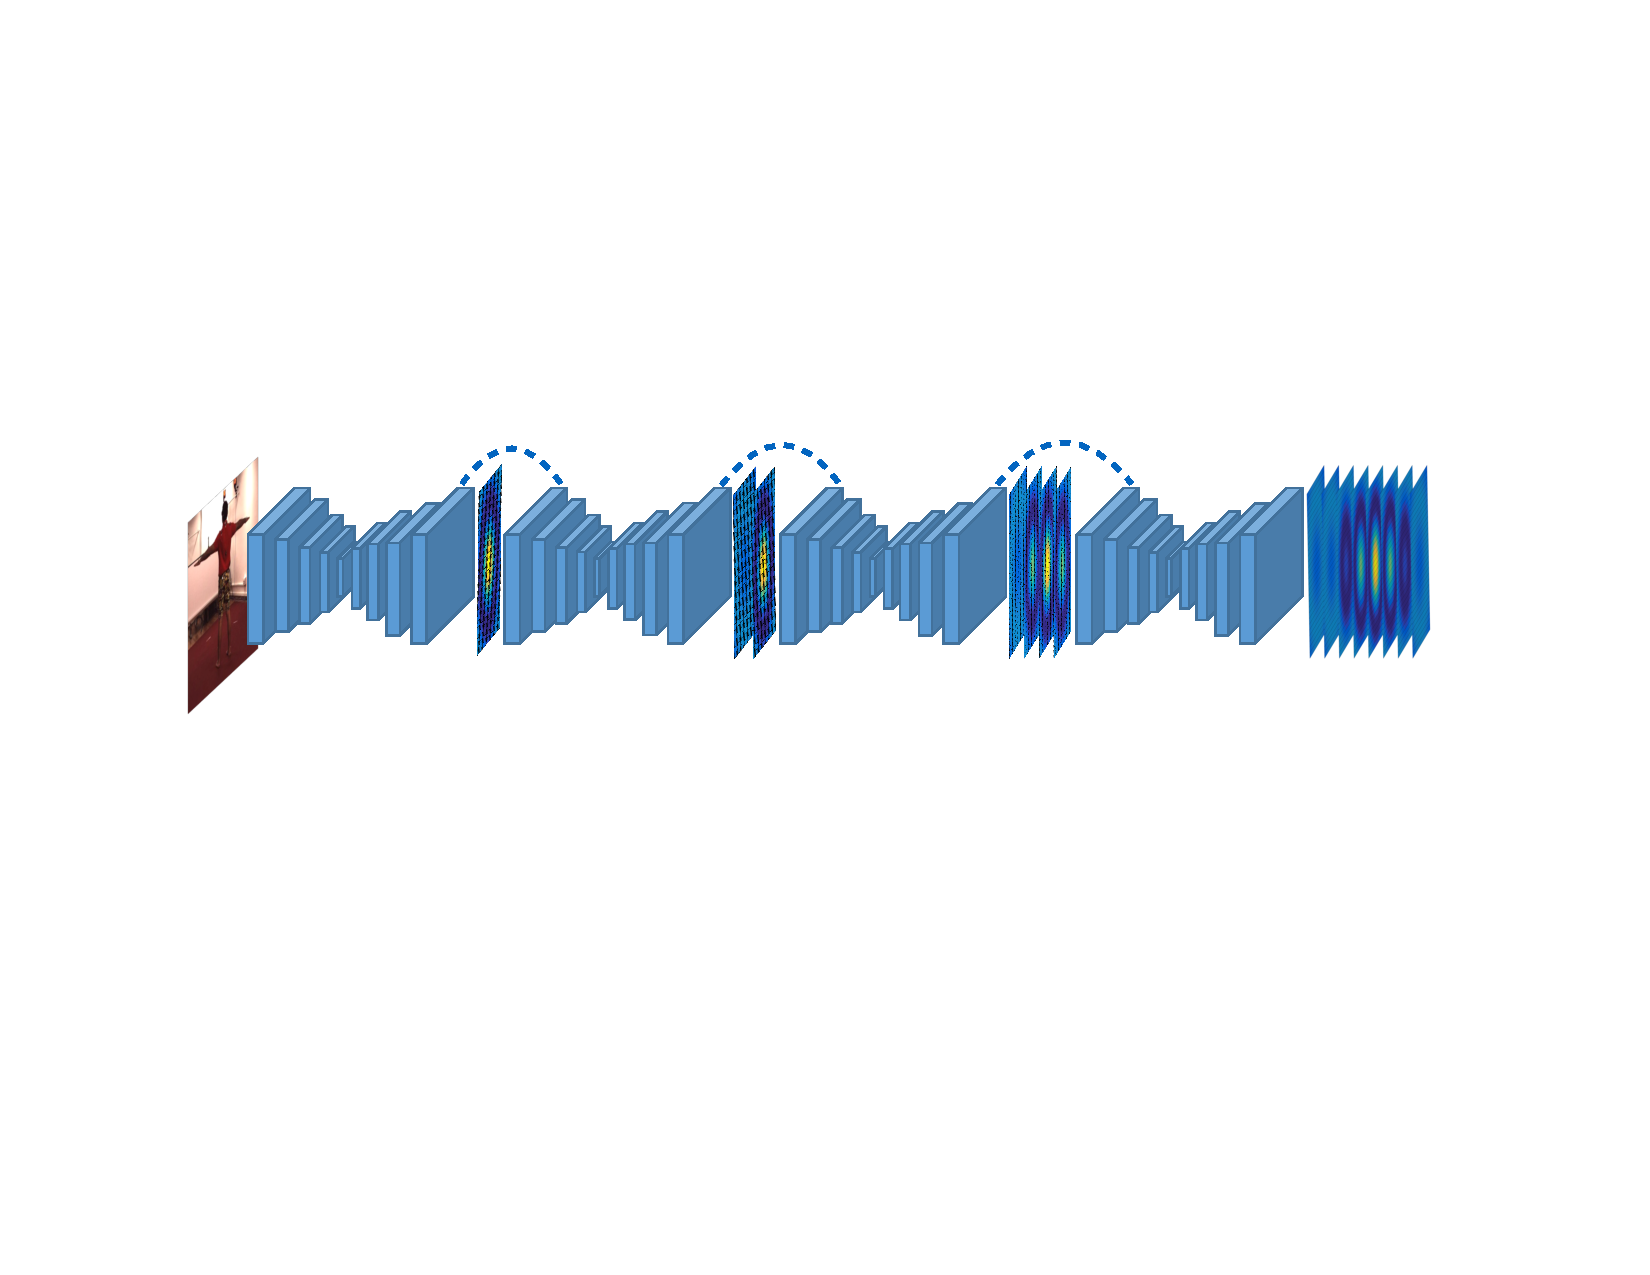
\includegraphics[width=1\linewidth,trim={2.7cm 9.5cm 3.5cm 7.4cm},clip]{review/coarse-to-fine.pdf}
    \caption{由粗到细\autocite{pavlakos2017coarse}:从输入图片中去估计每个关节的深度,深度方向的分辨率由粗到细}\label{fig:c2f}
\end{figure}

当下有一些文献认为仅仅用 3D 骨架的方法来描述 3D 姿态过于简单, Bogo等人\cite{bogo2016keep}提出了 SMPLify,一种基于优化的,从 14 个检测到的二维关节恢复SMPL 参数的方法。SMPL\autocite{loper2015smpl}是一种参数化表示的人体模型,这个模型从大量三维人体扫描数据中去学习人体的参数化表示,使得人们可以通过低维的参数去表示不通形状的人体模型。Bogo等人\cite{bogo2016keep}使用了优化的方法,将人体模型拟合到从图片中检测出来的二维人体关键点上。但是,由于加入了优化步骤,该方法不是实时的,每个图像需要 20-60 秒的时间进行处理。同时,由于从二维到三维的歧义性,他们在优化过程中加入了许多先验的知识,例如关节的角度的旋转范围,以及一个大量的姿势数据,使得得到的姿势接近数据库中的姿势。其部分结果如\refFig{fig:smpl1}所示。 

\begin{figure}[ht]
    \centering
    \includegraphics[width=1\linewidth]{review/smplify.pdf}
    \caption{Keep it SMPLify\autocite{bogo2016keep}:通过拟合SMPL人体模型到图片的二维关键点上}\label{fig:smpl1}
\end{figure}

Lassner \cite{lassner2017unite} 等人 从 SMPLify 的结果训练 91 个关键点探测器,其中一些相当于传统的身体关节,其他对应于身体表面的位置。然后,他们优化SMPL 模型参数以适应与\cite{bogo2016keep}类似的关键点。他们还提出了一种随机森林回归方法来直接回归 SMPL 参数,从而以精确性为代价减少运行时间,如\refFig{fig:up}所示。而近期Kanazawa 等人\cite{kanazawa2018end} 的方法直接从图像推断 SMPL 参数,而不依赖于检测到的 2D关键点,并且做到了实时运行。

\begin{figure}[ht]
    \centering
    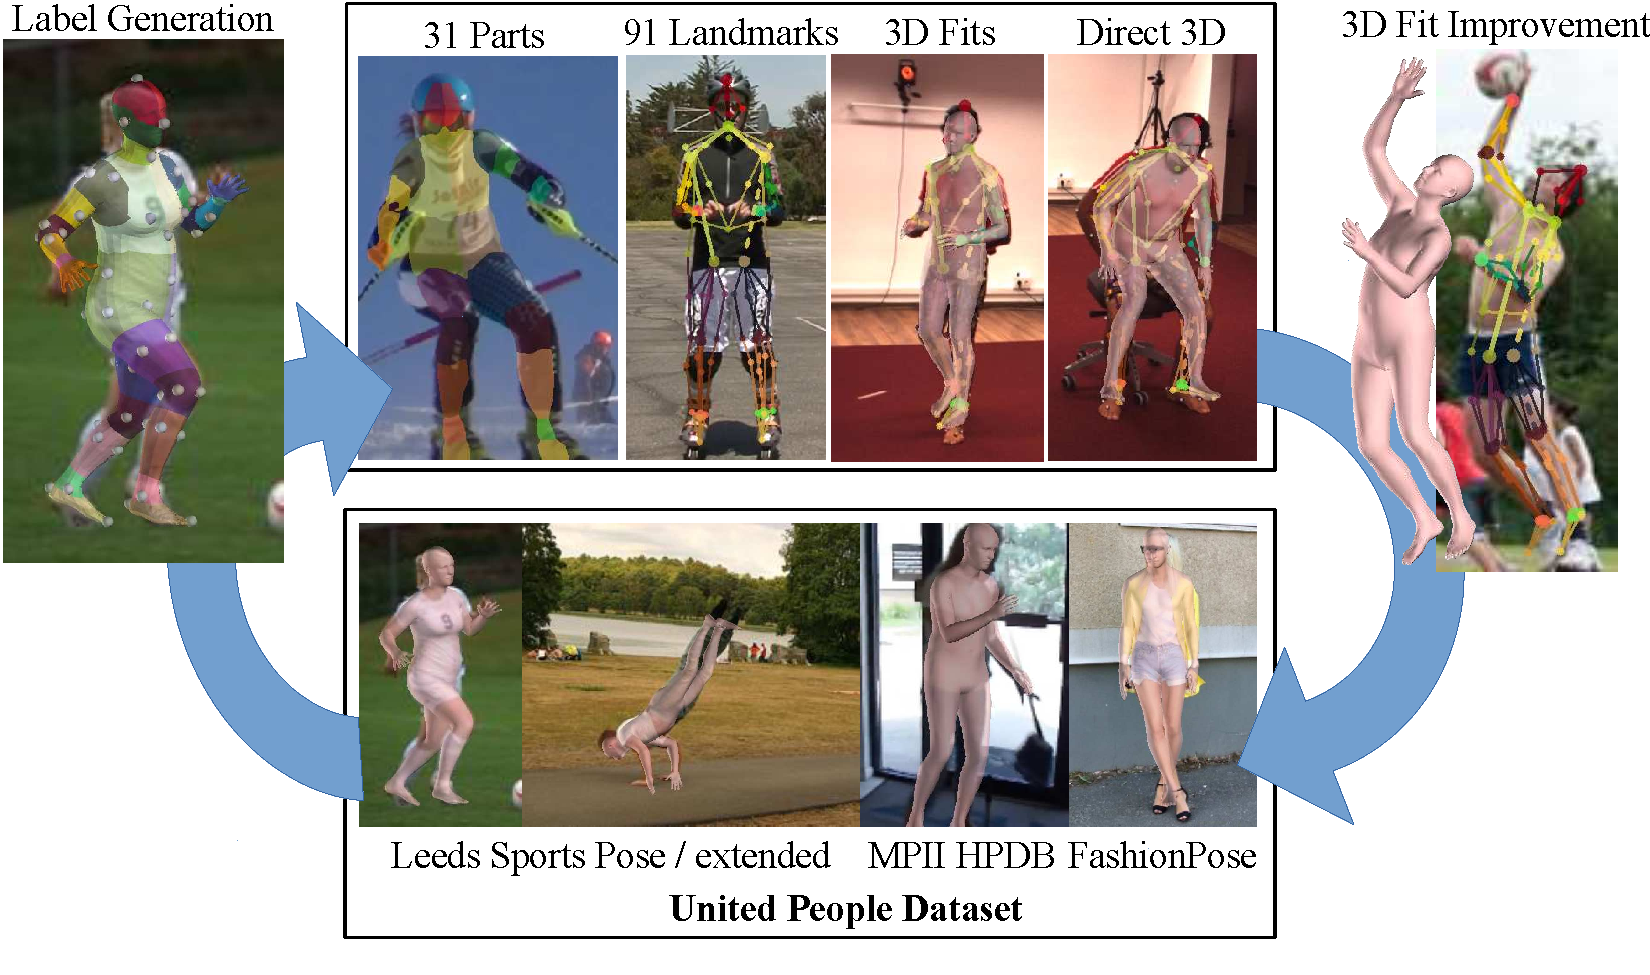
\includegraphics[width=1\linewidth]{review/up.pdf}
    \caption{Unit the people\autocite{lassner2017unite}:通过拟合SMPL模型到检测的人体的91个关节点上}\label{fig:up}
\end{figure}

% \section{研究展望}

\newpage
\printbibliography
\end{refsection}
